\section{Training and Result}
\label{sec:training-result}
%
The training process is execute at the university's HPC at the University of
Trento, with the aim of minimizing also the topics of this operation which is
particularly expensive in terms of calculation resources and time.
For this reason, it was decided to optimize the training procedure by modifying
only some of the parameters of interest, i.e. applying fine tuning techniques to
preserve the weights of a previous training and modifying only the input
layer and expand the final layer by adding new classification categories. 
The two most important parameters are:
\begin{itemize}
	\item Input image resolution: the corresponding value can be $128, 160, 192,
224$ pixels or greater. In this project, a size of $512$ pixels was chosen, this
in order not to penalize excessively the input images. At high altitudes, as
explained for the realization of the dataset in section (\ref{ssec:landing-zone}),
the details and targets becoming extremely difficult to detect therefore a high
scaling worsens the result. Meanwhile this choice negatively affects the
duration of the entire training by lengthening the processing times.
	\item The second parameter relating to the model: this value allows you to
establish the size of the model starting from the complete one, i.e. it is
possible to train a fraction of the model, choosing from the values: $1, 0.75,
0.50$ or $0.25$. The higher the fraction chosen, the greater the precision of
the model.
\end{itemize}
%
\begin{listing}[ht] 
\inputminted[frame=lines,framesep=2mm, linenos=true, autogobble, breaklines=true, fontsize=\scriptsize, firstline=25, lastline=38]{shell}{neuralnetworks/code/train_ssd_mobilenet_v2_coco_2018_03_29.sh} 
\caption{Train script setup.} 
\label{lst:train-code-shell} 
\end{listing}
%
The above commands (\ref{lst:train-code-shell}) are used to set the selected
model, the folder of the dataset containing the images, the labels of the target
objects and the destination folder of the trained model.
The \texttt{num\_train\_steps} parameter set to $50000$ indicates how many times
training iterates over data. The higher this value, the more accurate the result
will be.
%
\subsection{Result}
\label{ssec:result}
%
In the graphs shown in the figures (\ref{fig:training-1}, \ref{fig:training-2}) it is
possible to observe the progress of the training process on the quantities of
interest. In particular we observe that:
\begin{itemize}
	\item \textbf{\texttt{rpn\_class\_loss}} RPN anchor classifier loss;
	\item \textbf{\texttt{rpn\_bbox\_loss}} RPN bounding box loss graph;
	\item \textbf{\texttt{class\_loss}} loss for the classifier head of CNN;
	\item \textbf{\texttt{bbox\_loss}} loss for bounding box refinement;
\end{itemize}
Each of these loss metrics is the sum of all the loss values calculated
individually for each of the regions of interest.
The general loss metric given in the log is the sum of the other five losses
(it possible check it by summing them up).
The values of the classification losses depend on the confidence value
associated with the real class. 
Consequently, these values reflect the confidence of the model in predicting and
labelling a class, that is, verifying how correct the prediction is.\\
The bounding box loss values reflect the distance between the true box
parameters that is, the $(x, y)$ coordinates of the box location, its width and
its height and the predicted ones.
This value derives from the loss of regression and penalizes major absolute
differences. 
In particular, it will exhibit a behaviour for small differences, on the other
hand a linear compaction for large differences. Ultimately this aspect reveals
to us how correct the localization of the objects within the image is, that is,
this value allows us to evaluate how precisely the model foresees the area that
contains the object.
This information is extracted by TensorBoard is another great debugging and
visualization tool. 
The model is configured to log losses and save weights at the end of every
epoch.\cite{matterport_maskrcnn_2017}
%
\begin{figure}[h!]
  \begin{center}
  \begin{tikzpicture}
  \begin{axis}[width=12cm, height=7cm,  grid=major, grid style={dashed,gray!30},
    xlabel=epoch,  ylabel=loss, legend pos=outer north east, legend cell align=left, smooth]
		\addplot[red] 			table [x=step, y=val_loss, col sep=comma] 				{neuralnetworks/scalars.csv};
		\addlegendentry{{\scriptsize val loss}}
		\addplot[babyblueeyes] 	table [x=step, y=mrcnn_class_loss, col sep=comma] 		{neuralnetworks/scalars.csv};
		\addlegendentry{{\scriptsize class loss}}
		\addplot[amber] 		table [x=step, y=val_rpn_bbox_loss, col sep=comma] 	{neuralnetworks/scalars.csv};
		\addlegendentry{{\scriptsize rpn bounding box}}
		\addplot[amethyst] 		table [x=step, y=rpn_class_loss, col sep=comma] 		{neuralnetworks/scalars.csv};
		\addlegendentry{{\scriptsize rpn class loss}}
		\addplot[black] 		table [x=step, y=rpn_bbox_loss, col sep=comma] 		{neuralnetworks/scalars.csv};
		\addlegendentry{{\scriptsize rpn boundig box}}
		\addplot[applegreen] 	table [x=step, y=val_mrcnn_class_loss, col sep=comma] 	{neuralnetworks/scalars.csv};
		\addlegendentry{{\scriptsize val class loss}}
		\addplot[bananayellow] 	table [x=step, y=val_rpn_class_loss, col sep=comma] 	{neuralnetworks/scalars.csv};
		\addlegendentry{{\scriptsize val rpn class loss}}
		\addplot[violet] 	table [x=step, y=val_mrcnn_bbox_loss, col sep=comma] 	{neuralnetworks/scalars.csv};
		\addlegendentry{{\scriptsize val bounding box}}
		\addplot[beaver] 		table [x=step, y=mrcnn_bbox_loss, col sep=comma] 		{neuralnetworks/scalars.csv};
		\addlegendentry{{\scriptsize bounding box loss}}
		\addplot[ceruleanblue] 	table [x=step, y=loss, col sep=comma] 					{neuralnetworks/scalars.csv};
		\addlegendentry{{\scriptsize loss}}
	\end{axis}
\end{tikzpicture}
\caption{Result training object detection on last ouptut layer.}
\label{fig:training-1}
\end{center}
\end{figure}
%
\begin{figure}[h!]
  \begin{center}
  \begin{tikzpicture}
  \begin{axis}[width=12cm, height=7cm,  grid=major, grid style={dashed,gray!30},
    xlabel=epoch,  ylabel=loss, legend pos=outer north east, legend cell align=left, smooth]
		\addplot[red] 			table [x=step, y=val_loss, col sep=comma] 				{neuralnetworks/scalars100-199.csv};
		\addlegendentry{{\scriptsize val.}}
		\addplot[babyblueeyes] 	table [x=step, y=mrcnn_class_loss, col sep=comma] 		{neuralnetworks/scalars100-199.csv};
		\addlegendentry{{\scriptsize mclass loss}}
		\addplot[amber] 		table [x=step, y=val_rpn_bbox_loss, col sep=comma] 		{neuralnetworks/scalars100-199.csv};
		\addlegendentry{{\scriptsize rpn boundin box loss}}
		\addplot[amethyst] 		table [x=step, y=rpn_class_loss, col sep=comma] 		{neuralnetworks/scalars100-199.csv};
		\addlegendentry{{\scriptsize rpn class loss}}
		\addplot[black] 		table [x=step, y=rpn_bbox_loss, col sep=comma] 			{neuralnetworks/scalars100-199.csv};
		\addlegendentry{{\scriptsize rpn boundig box loss}}
		\addplot[applegreen] 	table [x=step, y=val_mrcnn_class_loss, col sep=comma] 	{neuralnetworks/scalars100-199.csv};
		\addlegendentry{{\scriptsize val class loss}}
		\addplot[bananayellow] 	table [x=step, y=val_rpn_class_loss, col sep=comma] 	{neuralnetworks/scalars100-199.csv};
		\addlegendentry{{\scriptsize val rpn class loss}}
		\addplot[violet] 	table [x=step, y=val_mrcnn_bbox_loss, col sep=comma] 	{neuralnetworks/scalars100-199.csv};
		\addlegendentry{{\scriptsize val bounding box loss}}
		\addplot[beaver] 		table [x=step, y=mrcnn_bbox_loss, col sep=comma] 		{neuralnetworks/scalars100-199.csv};
		\addlegendentry{{\scriptsize bounding box loss}}
		\addplot[ceruleanblue] 	table [x=step, y=loss, col sep=comma] 					{neuralnetworks/scalars100-199.csv};
		\addlegendentry{{\scriptsize loss}}
	\end{axis}
\end{tikzpicture}
\caption{Result training classification.}
\label{fig:training-2}
\end{center}
\end{figure}
%
%
\newpage
Finally, some examples of inference are given to evaluate the response of the
trained model as can be seen in figures (\ref{fig:evaluation}). 
Although images taken from the internet have been provided and taken from real
environments using some demonstrations that those generated by the computer; the
model is able to provide the correct answer even when the target object is
covered with elements.
\begin{figure}[htb]
    \centering
    \subfloat[][\emph{product image}]{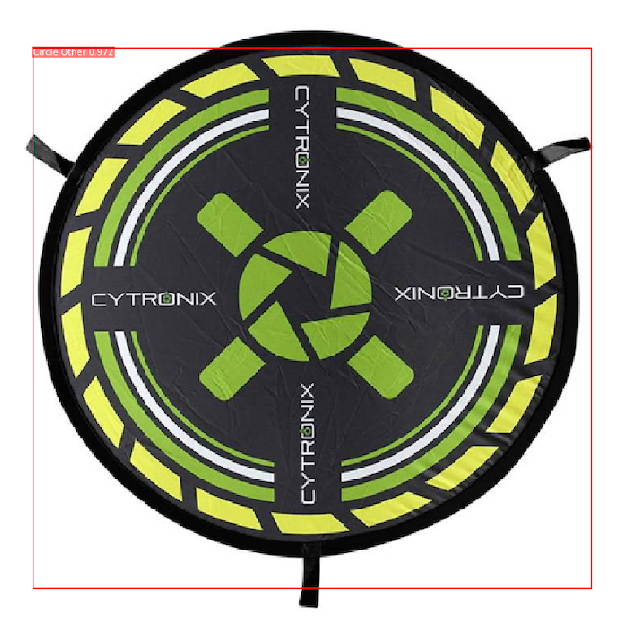
\includegraphics[width=.45\textwidth]{test1.png}} 	\quad
    \subfloat[][\emph{real environment - grass}]{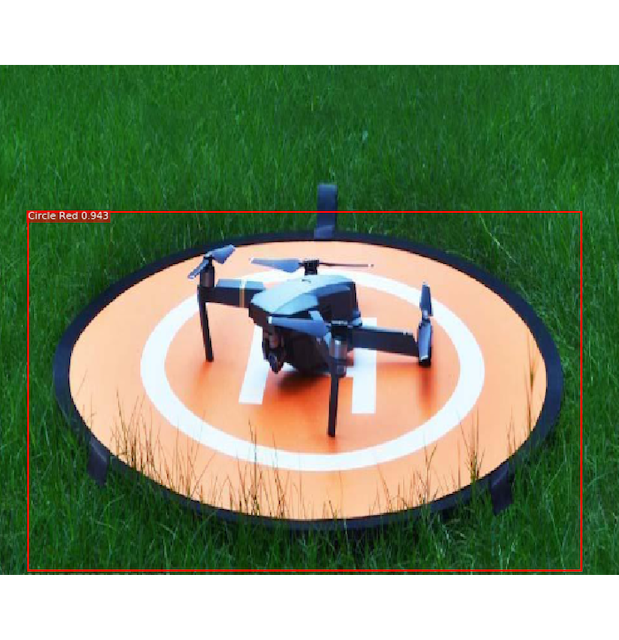
\includegraphics[width=.45\textwidth]{test3.png}} 	\\
    \subfloat[][\emph{real environment - sand}]{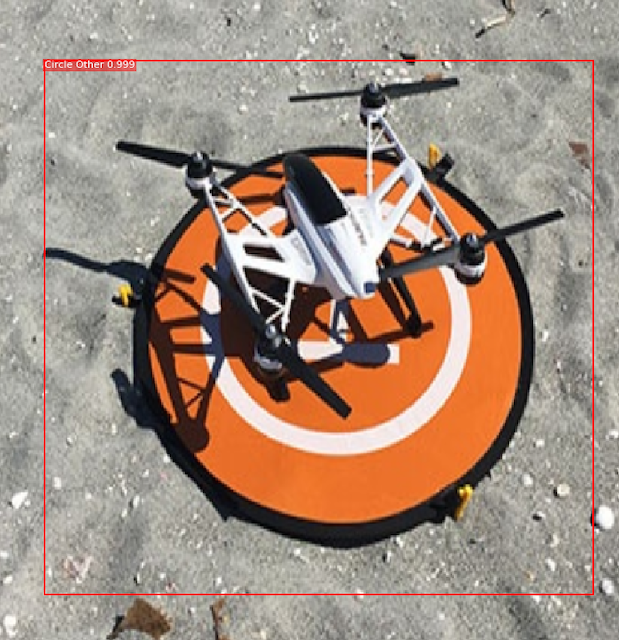
\includegraphics[width=.45\textwidth]{test4.png}}	\quad
    \subfloat[][\emph{render from dataset}]{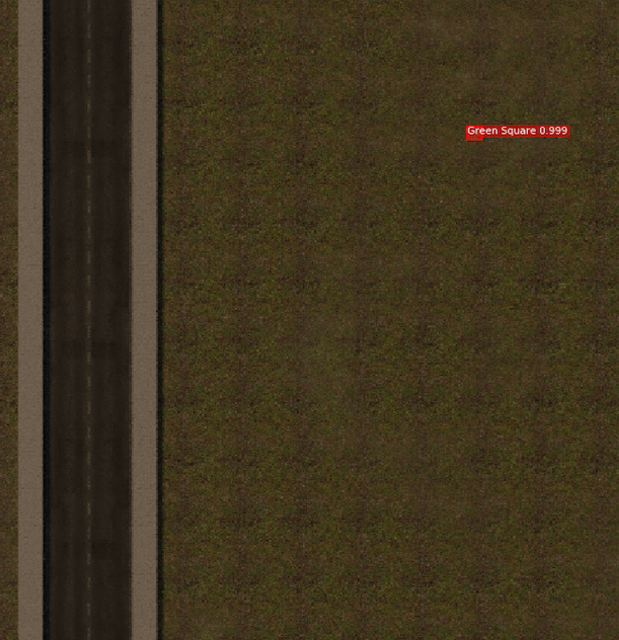
\includegraphics[width=.45\textwidth]{test5.png}}
    \caption{Evaluation of the model response with images.}
    \label{fig:evaluation}
\end{figure}
